\documentclass[10pt]{article}
\usepackage{geometry}
\geometry{a4paper}
\pagestyle{myheadings}
\usepackage{tikz}
\usepackage{pgfplots}
\usepackage{fancyhdr} % Required for custom headers
\usepackage{lastpage} % Required to determine the last page for the footer
\usepackage{extramarks} % Required for headers and footers
\usepackage{graphicx} % Required to insert images
\usepackage{listings} % Required for insertion of code
\usepackage{courier} % Required for the courier font
\usepackage{caption}
\usepackage{subcaption}
\usepackage{amsmath}
\usepackage{amsfonts}
\usepackage{amssymb}
\usepackage{epstopdf}
\usepackage{placeins}
\usepackage{fancyvrb} 
\usepackage[numbered]{bookmark}
\usepackage{pgfplots}
\usepackage{ifthen}
\usepackage{setspace}
\usepackage{placeins} % for FloatBarrier
\usepackage[makeroom]{cancel}
\usepackage[absolute,overlay]{textpos}
\usetikzlibrary{calc, angles,quotes}
\usetikzlibrary{pgfplots.fillbetween, backgrounds}
\usetikzlibrary{positioning}
\usetikzlibrary{arrows}
\usetikzlibrary{pgfplots.groupplots}
\usetikzlibrary{arrows.meta}
\usetikzlibrary{plotmarks}
\usetikzlibrary{decorations.markings}

\usepgfplotslibrary{groupplots}
\pgfplotsset{compat=newest} 

\DeclareGraphicsExtensions{.pdf,.png,.jpg}
\graphicspath{{../figs/}}

\definecolor{blue2}{RGB}{51, 105, 232}  
\definecolor{red2}{RGB}{213, 15, 37}  
\definecolor{green2}{RGB}{0, 153, 37}  

\definecolor{matlabcomment}{RGB}{34,139,34}

\pgfmathdeclarefunction{gauss}{1}{%
	\pgfmathparse{1/(sqrt(2*pi))*exp(-((#1)^2)/2)}%
}

\pgfmathdeclarefunction{laplacian}{2}{%
	\pgfmathparse{1/(#2*2)*exp(-(abs(x-#1))/(#2))}%
}

\pgfmathdeclarefunction{pretty_func}{1}{%
	\pgfmathparse{cos(deg(#1/2)) - sin(deg(#1)) + cos(deg(#1/2)-45) - sin(deg(#1/4)-154)}%
}

\pgfplotsset{
	dirac/.style={
		mark=triangle*,
		mark options={scale=2},
		ycomb,
		scatter,
		visualization depends on={y/abs(y)-1 \as \sign},
		scatter/@pre marker code/.code={\scope[rotate=90*\sign,yshift=-2pt]}
	}
}

\def\thickness{very thick}

\tikzset{
amark/.style 2 args={
	decoration={             
		markings, 
		mark=at position {0.5} with { 
			\arrow{stealth},
			\node[#2] {#1};
		}
	}, \thickness,
	postaction={decorate}
},
earlymark/.style 2 args={
	decoration={             
		markings, 
		mark=at position {0.25} with { 
			\arrow{stealth},
			\node[#2] {#1};
		}
	}, \thickness,
	postaction={decorate}
},
latemark/.style 2 args={
	decoration={             
		markings, 
		mark=at position {0.8} with { 
			\arrow{stealth},
			\node[#2] {#1};
		}
	}, \thickness,
	postaction={decorate}
},
zpath/.style={
	decoration={             
		markings, 
		mark=at position {0.5} with { 
			\arrow{stealth},
			\node[#1] {$z^{-1}$};
		}
	}, \thickness,
	postaction={decorate}
},
terminal/.style 2 args={draw,circle,inner sep=2pt,label={#1:#2}},
}


\tikzset{
	invisible/.style={opacity=0},
	visible on/.style={alt={#1{}{invisible}}},
	alt/.code args={<#1>#2#3}{%
		\alt<#1>{\pgfkeysalso{#2}}{\pgfkeysalso{#3}} % \pgfkeysalso doesn't change the path
	},
}

\newcommand\PlotSampledSpectrum[4]{%
	\def\fs{#2}%
	\def\fmax{#3}%
	\def\ros{#4}%
	\input{#1}%
}

\pgfmathdeclarefunction{invgauss}{2}{%
	\pgfmathparse{sqrt(-2*ln(#1))*cos(deg(2*pi*#2))}%
}

\tikzset{
	declare function={
		sinc(\x) = (and(\x!=0, 1) * (sin(deg(pi*\x))/(pi*\x)) +
		(and(\x==0, 1) * 1);
	}
}

%\DeclareMathOperator{\E}{\mathbb{E}} % expectation

\newcommand\SimpleSys[4]{%
	\def\xin{#2}%
	\def\Hz{#3}%
	\def\yout{#4}
	\input{#1}%
}

%%%%%%%%%%%%% SOLUTIONS %%%%%%%%%%%%%%%%%
\def\SOLUTIONS{1} % change to 1 to produce solutions
\def\SolutionsColor{red2}
%%%%%%%%%%%%%%%%%%%%%%%%%%%%%%%%%%%%%%%%%

% Header
\if\SOLUTIONS1
	\markboth{\em \color{\SolutionsColor} \textbf{EE264: Final exam solutions}}{\em \color{\SolutionsColor} \textbf{EE264: Final exam solutions}}
    \title{EE 264 Final exam solutions}
\else
	\markboth{\em EE264: Midterm, August 1st -- Summer 2017}{\em EE264: Final, Summer 2017}
    \title{EE 264 Final}
\fi

% Document
\begin{document}
\doublespacing
\begin{center}
\textbf{\Large Stanford University}

\textbf{\Large Department of Electrical Engineering}

\Large EE 264: Digital Signal Processing 

\Large Final Exam

\Large Summer, 2018
\end{center}
\vspace{-0.5cm}
\rule{\textwidth}{1pt}

\noindent\textbf{Name:} \rule{0.4\textwidth}{0.5pt} \qquad  \textbf{Date and time:} \rule{0.3\textwidth}{0.5pt}

\noindent\textbf{SUNet ID:} \rule{0.3\textwidth}{0.5pt}\qquad 
\textbf{SCPD Student?} yes no

\mbox{}\\
\textbf{Instructions:}
\singlespacing
\begin{enumerate}
\item This is a 24h-take home exam. 
\item Carefully read over and understand the exam problems before you start.
\item The exam is open book and open notes. You may use all available references.
\item Be clear, organized, and concise in your answers.
\item During grading we will not propagate errors. We will evaluate your answers to each question independently from previous answers.
\item Please submit your solutions in a single .pdf file on Gradescope. Your solutions \underline{must} include derivations, clearly labeled plots, and code you developed. Your submission \underline{must} also include this cover page signed. 
\item Do \underline{not} communicate with others about the exam even after you have taken it, as some students will take the exam at a different time.
\item Do \underline{not} post questions on Piazza during the exam. If you have questions, please contact the teaching staff \{anchit, jkperin\}@stanford.edu. However, we will not provided additional hints or check your answers.
\end{enumerate}

\noindent\textbf{The Stanford University Honor Code:}
\begin{quote}
I attest that I have not given or received aid in this examination, and that I have done my share and taken an active part in seeing to it that others as well as myself uphold the spirit and letter of the Honor Code.
\end{quote}
\vspace{1mm}

\begin{center}\textbf{Signature:} \rule{0.7\textwidth}{0.5pt}\end{center}

\doublespacing
\vspace{0.1cm}
\begin{center}
\begin{tabular}{ccc}
\textbf{Problem} & \textbf{Points} & \textbf{Score} \\
1 & 60 & \\
2 & 60 & \\
\end{tabular}
\end{center}
\singlespacing
\pagebreak

\section*{Problem 1: Hearing aid (55 points)}

Figure~\ref{fig:hearing_aid_diagram} shows the block diagram of a hearing aid device. The signal recorded by the microphone is low-pass filtered by the anti-aliasing filter $H_{aa}(j\Omega)$, and then converted to digital domain by the ADC. A digital filter $H(z)$ corrects for the patient's hearing loss by boosting the signal at particular frequencies or band of frequencies. Once the signal has been filtered, it is converted back to the analog domain using a DAC, which will then drive a speaker that is placed inside the patient's hearing canal. 

\FloatBarrier
\begin{figure}[h!]
	\centering
	\resizebox{\textwidth}{!}{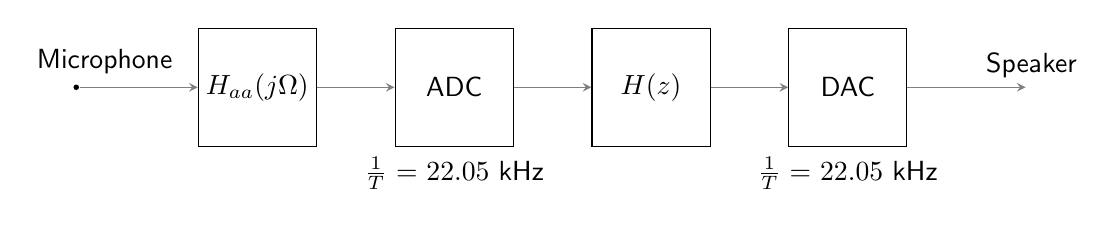
\begin{tikzpicture}[->, >=stealth, shorten >= 0pt, draw=black!50, node distance=2.5cm, font=\sffamily]
    \tikzstyle{node}=[circle,fill=black,minimum size=2pt,inner sep=0pt]
    \tikzstyle{block}=[draw=black,rectangle,fill=none,minimum size=1.5cm, inner sep=0pt]

	\node[node] (xc) {};
	\node[block, right=1.5cm of xc] (Haa) {$H_{aa}(j\Omega)$};
    \node[block, right of=Haa] (ADC) {ADC};
    \node[block, right of=ADC] (DSP) {$H(z)$};
    \node[block, right of=DSP] (DAC) {DAC};
	\coordinate[right=1.5cm of DAC] (yc) {};
		
    \path (xc) edge (Haa);
    \path (Haa) edge (ADC);
    \path (ADC) edge (DSP);
    \path (DSP) edge (DAC);
    \path (DAC) edge (yc);
    
    \node[above = 0mm of xc, text width = 1cm, align=center] {Microphone};
    \node[above = 0mm of yc, text width = 1cm, align=center] {Speaker};
    \node[below, align=center, text width=2.5cm] at ($(ADC.south)$) {$\frac{1}{T} = 22.05$ kHz};
    \node[below, align=center, text width=2.5cm] at ($(DAC.south)$) {$\frac{1}{T} = 22.05$ kHz};
\end{tikzpicture}}
	\caption{Block diagram of a digital hearing aid device.}
	\label{fig:hearing_aid_diagram}
\end{figure}
\FloatBarrier

\FloatBarrier
\begin{figure}[h!]
	\centering
	\resizebox{0.7\textwidth}{!}{\begin{tikzpicture}
\begin{axis}[
%axis lines*=middle,
enlargelimits = false, clip=true,
scale only axis,
axis line style={->,>=stealth, shorten >= 0pt},
xlabel={Frequency (Hz)},
ylabel={Hearing loss (dB)},
every outer x axis line/.append style={white!15!black},
every x tick label/.append style={font=\color{white!15!black}},
xmin=0, xmax=10,
ymin=-60, ymax=10,
xtick={0.5, 1, 2, 3, 4, 5, 6, 7, 8, 9, 10},
ymajorgrids,
xmajorgrids,
every outer y axis line/.append style={white!15!black},
every y tick label/.append style={font=\color{white!15!black}},
legend style={draw=white!15!black,fill=white,legend cell align=left, at={(axis cs: 1.05, -5)}}]

\addplot [smooth, color=black, mark=*, mark size = 3pt, mark options={fill=white}, solid, line width=2pt] table[x index=0,y index=1] {figs/adiogram.dat}; 

\end{axis}
\end{tikzpicture}


% each nth point={100}
% restrict x to domain=1:4}
	\caption{Audiogram of patient.}
	\label{fig:audiogram}
\end{figure}
\FloatBarrier

Figure~\ref{fig:audiogram} shows the \textit{audiogram} of a given patient. This plot shows the patient's hearing loss at particular frequencies. For instance, a hearing loss of 0 dB means that no correction needs to be done at that frequency. However, this patient has a hearing loss of 50 dB at 10 kHz. Hence, the system must provide a gain of nearly 50 dB at 10 kHz. The data from this plot is available in the file \texttt{hearing\_aid.m}. 

For the following questions assume that the sampling rate of the ADC is $1/T = 22.05$ kHz, and the same sampling period is used for reconstruction.
\begin{description}
	\item[(a)] (3 points) Plot the desired filter specification $|H_d(e^{j\omega})|$ that would compensate for the patient's hearing loss. The $x$-axis of your plot should be the normalized frequency $\omega$ or $\omega/\pi$, while the $y$-axis should be the magnitude $20\log_{10}(|H_d(e^{j\omega})|)$ in dB.
	
	\if\SOLUTIONS1
	{\color{\SolutionsColor} The filter specification is simply the inverse of the patient's hearing loss.
	
	\FloatBarrier
	\begin{figure}[h!]
		\centering
		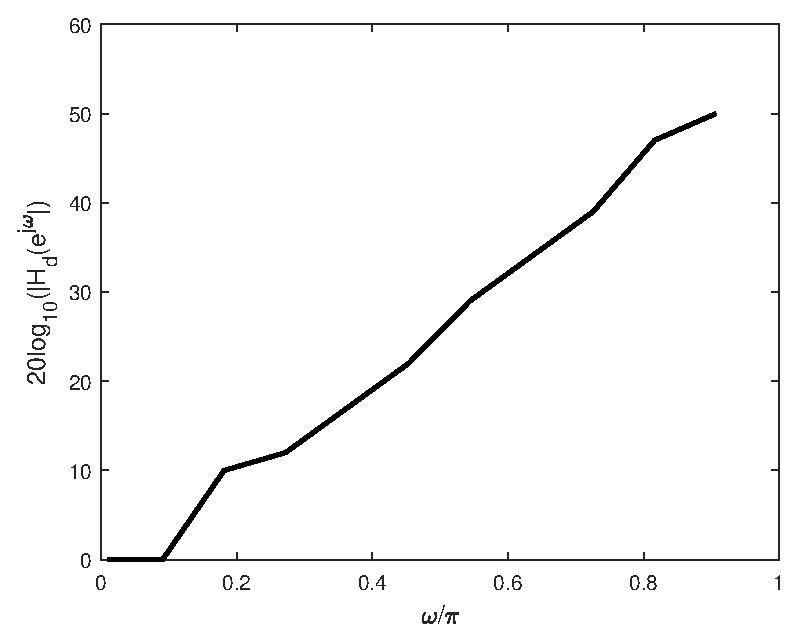
\includegraphics[scale=0.6]{figs/hearing_aid_spec.eps}
		\caption{Filter specification for correction of the patient's hearing loss.}
	\end{figure}
	\FloatBarrier
	}
	\fi
	
	\item[(b)] (5 points) The reconstruction filter of the DAC is a linear interpolator. This filter causes an additional attenuation given by
	\begin{equation}
		H_{DAC}(j\Omega) = \mathrm{sinc}^2\Big(\frac{\Omega}{2\pi}T\Big), \quad |\Omega| \leq \frac{\pi}{T}
	\end{equation}
	Adjust the filter specification $|H_d(e^{j\omega})|$ calculated in part (a) so that the filter $H(z)$ would also compensate for the attenuation introduced by the DAC. Plot the adjusted specification. Once again, the $x$-axis of your plot should be normalized frequency $\omega$ or $\omega/\pi$, while the $y$-axis should be the magnitude $20\log_{10}(|H_d(e^{j\omega})|)$ in dB.
	
	\noindent\textit{Note:} In the DSP literature, pre-compensating for a filter response is called \textit{pre-emphasis}. In this question, you're performing pre-emphasis to compensate for the patient's hearing loss and also for the non-ideal reconstruction filter.
	
	\if\SOLUTIONS1
	{\color{\SolutionsColor} The corrected filter specification is given by
		\begin{equation*}
			|H_d(e^{j\omega})| = \frac{1}{|A(e^{j\omega})|\mathrm{sinc}^2(\frac{\omega}{2\pi})},
		\end{equation*}
		where $|A(e^{j\omega})|$ is patient's audiogram response. At the highest frequencies, the DAC causes about 8 dB of additional attenuation.
		
		\FloatBarrier
		\begin{figure}[h!]
			\centering
			\includegraphics[scale=0.6]{figs/hearing_aid_corrected_spec.eps}
			\caption{Corrected filter specification that accounts for the DAC attenuation.}
		\end{figure}
		\FloatBarrier
	}
	\fi
		
	\item[(c)] (15 points) Using your specification from part (b), design a generalized \underline{linear-phase} filter $H(z)$ that will approximate $|H_d(e^{j\omega})|$. Select the filter order so that the error between the desired response $H_d(e^{j\omega})$ and your design is \underline{at most} 1 dB at all frequencies. Plot $20\log_{10}(|H_d(e^{j\omega})|/|H(e^{j\omega})|)$ to show that your filter meets this specification. Additionally, plot the magnitude and phase response of your filter. 
	
	\if\SOLUTIONS1
	{\color{\SolutionsColor} Using the least-squares method, the filter that meets the specification to within 1 dB has order $M = 37$. Other answers obtained through the least-squares or Parks-McClellan method are accepted as long as the error is smaller than 1 dB at all frequencies.
		
	\FloatBarrier
	\begin{figure}[h!]
		\centering
		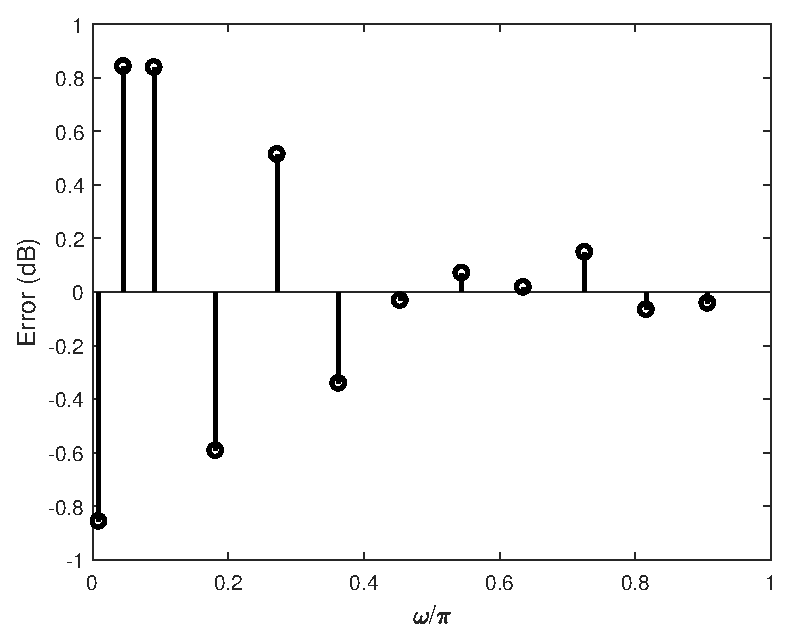
\includegraphics[scale=0.6]{figs/hearing_aid_filter_error.eps}
		\caption{Magnitude difference between the designed FIR filter and the specification from part (b). The error is smaller than 1 dB at all given frequencies. The filter order is $M = 37$.}
	\end{figure}
	\FloatBarrier	
	
	The frequency and phase response of filter is shown below
	\FloatBarrier
	\begin{figure}
		\centering
		\begin{subfigure}[h!]{0.5\textwidth}
			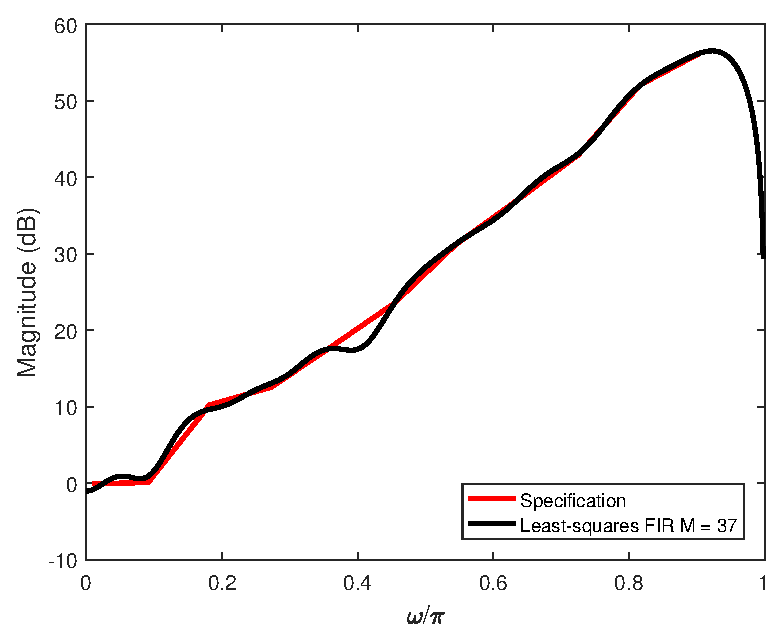
\includegraphics[scale=0.55]{figs/hearing_aid_filter_mag.eps}
			\caption{Magnitude}
		\end{subfigure}~\begin{subfigure}[h!]{0.5\textwidth}
			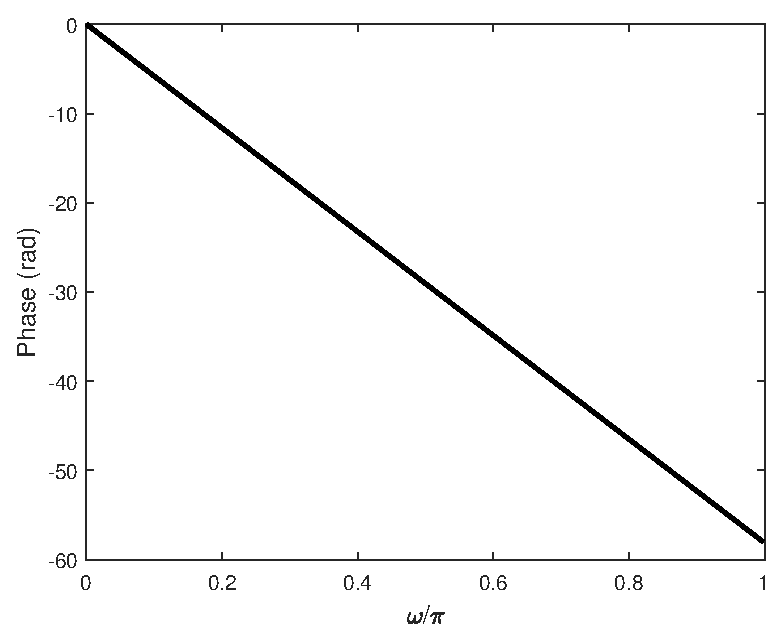
\includegraphics[scale=0.55]{figs/hearing_aid_filter_phase.eps}
			\caption{Phase}
		\end{subfigure}
		\caption{(a) magnitude and (b) phase of FIR filter of order $M = 37$ designed by the least-squares algorithm.}
	\end{figure}
	\FloatBarrier	
	}
	\fi
	
	\item[(d)] (3 points) Assuming that your filter is the only cause of delay in the system, what is the time difference between the time that the sound is recorded by the microphone and the time it is outputted by the speaker. Give your answers in samples and in seconds. 
	
	\if\SOLUTIONS1 {\color{\SolutionsColor} Since the filter is linear phase, it has equal group delay at all frequencies. The group delay is
		\begin{equation*}
			n_g = \frac{M}{2} = 18.5~\text{samples} \implies \tau_g = Tn_g = 0.839~\text{ms}
		\end{equation*}	
	}\fi

	\item[(e)] (7 points) Considering only quantization noise from the ADC, specify the minimum ADC resolution (in bits) so that the quantization noise average power \underline{after} $H(z)$ is at most $-30$ dBm (or 1 $\mu$W). Assume that the dynamic range of the quantizer is $\Delta X = 2$.
	
	\if\SOLUTIONS1 {\color{\SolutionsColor} Quantization noise has average power given by
		\begin{equation*}
			\sigma_Q^2 = \frac{\Delta^2}{12}, \quad \Delta = \frac{\Delta X}{2^B}
		\end{equation*}
		
		However, quantization noise is shaped by the filter $H(z)$. The noise average power after filtering is given by
		\begin{equation*}
			\sigma^2_{Q, out} = \sigma_Q^2\sum_{n = 0}^{M}|h[n]|^2 \tag{quantization noise shaping}
		\end{equation*}
		
		The output noise average power is smaller than $-30$ dBm (or $1 \mu$W) when $B = 18$, as can be verified in the plot below
		
		\FloatBarrier
		\begin{figure}[h!]
			\centering
			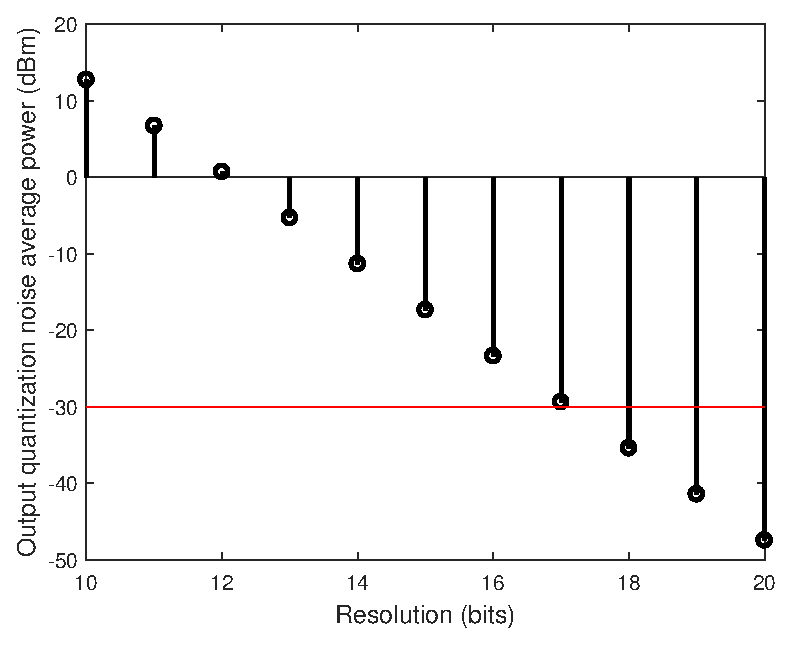
\includegraphics[scale=0.6]{figs/hearing_aid_quant_noise_var.eps}
			\caption{Average power of output quantization noise as a function of the resolution of the quantizer.}
		\end{figure}
		\FloatBarrier	
		
		Slightly different results may be obtained for different filters.
	}\fi
	
	\item[(f)] (7 points) Now include round-off noise from the filter implementation and determine the minimum ADC resolution (in bits) so that the \underline{total noise power} after $H(z)$ is at most $-30$ dBm (or 1 $\mu$W). Assume that the filter is implemented using the direct form I, and calculations are performed in two's complement using Q($B-1$) representation, where $B$ is the resolution of the ADC quantizer. Assume further that the result of multiplications is quantized \underline{immediately before} any additions are done. For the roundoff noise calculations assume that $X_m = 1$.
		
	\noindent\textit{Note:} Recall that in linear-phase implementations not all the coefficients need to be multiplied because of the symmetry in the impulse response.
	
	\if\SOLUTIONS1 {\color{\SolutionsColor} The number of required multiplications in a linear phase FIR filter is $\lfloor \frac{M}{2} + 1 \rfloor$. Therefore, the round-off noise resulting from rounding off the numbers immediately before additions is given by
	\begin{equation*}
		\sigma_{roundoff}^2 = \Big\lfloor \frac{M}{2} + 1 \Big\rfloor\frac{\Delta^2}{12}, \quad\Delta = \frac{X_m}{2^{B-1}}
	\end{equation*}
	Note that we use $B-1$ because the problem statement instructs us to use the Q($B-1$) representation, where $B$ is the number of bits of the ADC. In the lecture notes of roundoff noise, the quantizer had $B+1$ bits and we used the Q$B$ representation for numbers in the $[-1, 1]$ interval. 
	
	The roundoff noise is not shaped by the filter, hence the total noise average power after the $H(z)$ is given by
	\begin{equation*}
		\sigma^2_{total} = \sigma_Q^2\sum_{n = 0}^{M}|h[n]|^2 + \sigma_{roundoff}^2
	\end{equation*}
	
	The total noise average power after $H(z)$ is smaller than $-30$ dBm (or $1 \mu$W) when $B = 18$, as can be verified in the plot below
	
	\FloatBarrier
	\begin{figure}[h!]
		\centering
		\includegraphics[scale=0.6]{figs/hearing_aid_total_noise_var.eps}
		\caption{Total noise average power after $H(z)$ as a function of the resolution of the quantizer.}
	\end{figure}
	\FloatBarrier
	
		Slightly different results may be obtained for different filters.
	}\fi
	
		
	\item[(g)] (15 points) Now perform simulations to check whether your noise calculations are correct. In your simulations, you should include one white noise source to model quantization noise, and another white noise source to model round-off noise. These noise sources have to be \underline{zero mean} and have the appropriate \underline{average power}. Using any technique you prefer, estimate the PSD of the \underline{total noise} at the output of $H(z)$. On the same graph, plot the theoretical PSD and the estimated PSD. Use your result to estimate the average power of the noise and discuss whether it agrees with your theoretical estimates of part (e).
	
	\noindent\textit{Note:} Use the function \texttt{rand} to generate a white uniformly distributed noise, and use \texttt{filter} to filter the noise. Make sure that your noise sources are \underline{zero mean} and have the correct \underline{average power}.
	
	\if\SOLUTIONS1 {\color{\SolutionsColor}
		For the quantization noise, we need to generate an uniformly distributed zero-mean white noise signal with average power $\sigma_Q^2$, as calculated in part (e). For the roundoff noise, we need to generate an uniformly distributed zero-mean white noise signal with average power $\sigma_{roundoff}^2$, as calculated in part (f). The total noise will be given by
		\begin{equation}
			y[n] = h[n]\ast q[n] + r[n],
		\end{equation}
		where $q[n]$ is the quantization noise and $r[n]$ is the roundoff noise. Once we obtain the output noise $y[n]$ we can use Welch's method or the Blackman-Tukey method to estimate the PSD. These solutions assume the Blackman-Tukey method with Bartlett window of length $L = 2047$. See code for more details. The estimated PSD is plotted below
		
		\FloatBarrier
		\begin{figure}[h!]
			\centering
			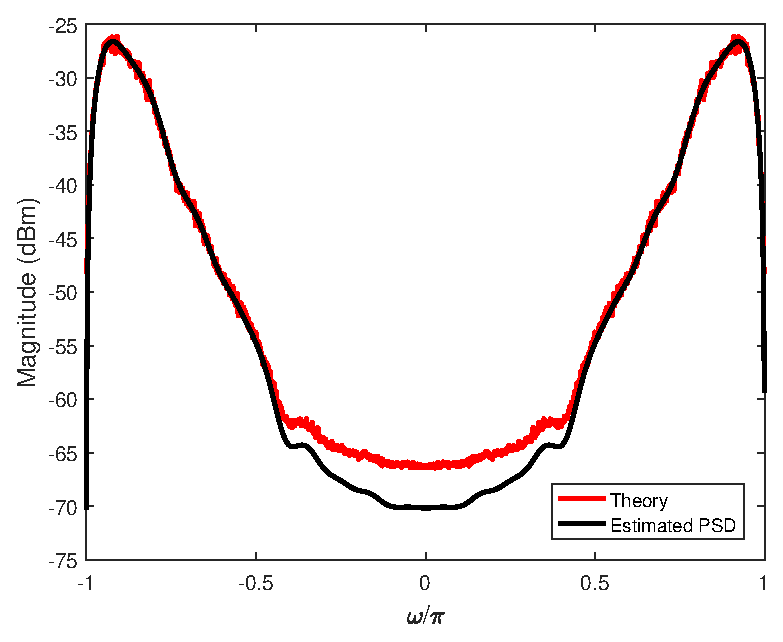
\includegraphics[scale=0.6]{figs/hearing_aid_psd.eps}
			\caption{Theoretical and estimated PSD. The PSD was estimated using the Blackman-Tukey method.}
		\end{figure}
		\FloatBarrier
		
		Note the error of the estimated PSD at small frequencies. To improve the accuracy we would need more samples. However, this error is not important, since the estimated power is nearly identical to the theoretical power. The estimated power is $-35.4977$. Hence, this design meets the specifications.
	}\fi
		
\end{description}

\if\SOLUTIONS1 
	\subsection*{Code for Problem 1}
	% This file was automatically created from the m-file 
% "m2tex.m" written by USL. 
% The fontencoding in this file is UTF-8. 
%  
% You will need to include the following two packages in 
% your LaTeX-Main-File. 
%  
% \usepackage{color} 
% \usepackage{fancyvrb} 
%  
% It is advised to use the following option for Inputenc 
% \usepackage[utf8]{inputenc} 
%  
  
% definition of matlab colors: 
\definecolor{mblue}{rgb}{0,0,1} 
\definecolor{mgreen}{rgb}{0.13333,0.5451,0.13333} 
\definecolor{mred}{rgb}{0.62745,0.12549,0.94118} 
\definecolor{mgrey}{rgb}{0.5,0.5,0.5} 
\definecolor{mdarkgrey}{rgb}{0.25,0.25,0.25} 
  
\DefineShortVerb[fontfamily=courier,fontseries=m]{\$} 
\DefineShortVerb[fontfamily=courier,fontseries=b]{\#} 
  
\noindent                                                                                                                                              
 \hspace*{-1.6em}{\scriptsize 1}$  $\color{mgrey}#%% Hearing aid problem #\color{black}$$\\
 \hspace*{-1.6em}{\scriptsize 2}$  clear, $\color{mdarkgrey}$clc, close all$\color{black}$$\\
 \hspace*{-1.6em}{\scriptsize 3}$  $\\
 \hspace*{-1.6em}{\scriptsize 4}$  T = 1/22.05e3;     $\color{mgrey}$% sampling time in seconds$\color{black}$$\\
 \hspace*{-1.6em}{\scriptsize 5}$  f = 1e3*[0.1 0.5 1 2 3 4 5 6 7 8 9 10]; $\color{mgrey}$% in Hz$\color{black}$$\\
 \hspace*{-1.6em}{\scriptsize 6}$  A = [0 0 0 -10 -12 -17 -22 -29 -34 -39 -47 -50]; $\color{mgrey}$% in dB$\color{black}$$\\
 \hspace*{-1.6em}{\scriptsize 7}$  $\\
 \hspace*{-1.6em}{\scriptsize 8}$  $\color{mgrey}#%% a)#\color{black}$$\\
 \hspace*{-1.6em}{\scriptsize 9}$  w_spec = 2*pi*f*T;$\\
 \hspace*{-2em}{\scriptsize 10}$  $\\
 \hspace*{-2em}{\scriptsize 11}$  $\color{mgrey}$% Plot results$\color{black}$$\\
 \hspace*{-2em}{\scriptsize 12}$  figure, $\color{mdarkgrey}$box on$\color{black}$$\\
 \hspace*{-2em}{\scriptsize 13}$  plot(w_spec/pi, -A, $\color{mdarkgrey}$'k'$\color{black}$, $\color{mdarkgrey}$'LineWidth'$\color{black}$, 2)$\\
 \hspace*{-2em}{\scriptsize 14}$  xlabel($\color{mdarkgrey}$'\omega/\pi'$\color{black}$, $\color{mdarkgrey}$'FontSize'$\color{black}$, 12)$\\
 \hspace*{-2em}{\scriptsize 15}$  ylabel($\color{mdarkgrey}$'20log_{10}(|H_d(e^{j\omega}|)'$\color{black}$, $\color{mdarkgrey}$'FontSize'$\color{black}$, 12)$\\
 \hspace*{-2em}{\scriptsize 16}$  axis([0 $\color{mdarkgrey}$1 0 60])$\color{black}$$\\
 \hspace*{-2em}{\scriptsize 17}$  saveas(gca, $\color{mdarkgrey}$'../figs/hearing_aid_spec'$\color{black}$, $\color{mdarkgrey}$'epsc'$\color{black}$)$\\
 \hspace*{-2em}{\scriptsize 18}$      $\\
 \hspace*{-2em}{\scriptsize 19}$  $\color{mgrey}#%% b)#\color{black}$$\\
 \hspace*{-2em}{\scriptsize 20}$  Hd = 1./(10.^(A/20).*sinc(w_spec/(2*pi)).^2);$\\
 \hspace*{-2em}{\scriptsize 21}$  figure, $\color{mdarkgrey}$plot(w_spec/pi, 20*log10(abs(Hd)))$\color{black}$$\\
 \hspace*{-2em}{\scriptsize 22}$  $\\
 \hspace*{-2em}{\scriptsize 23}$  $\color{mgrey}$% Plot results$\color{black}$$\\
 \hspace*{-2em}{\scriptsize 24}$  figure, $\color{mdarkgrey}$box on$\color{black}$$\\
 \hspace*{-2em}{\scriptsize 25}$  plot(w_spec/pi, 20*log10(abs(Hd)), $\color{mdarkgrey}$'k'$\color{black}$, $\color{mdarkgrey}$'LineWidth'$\color{black}$, 2)$\\
 \hspace*{-2em}{\scriptsize 26}$  xlabel($\color{mdarkgrey}$'\omega/\pi'$\color{black}$, $\color{mdarkgrey}$'FontSize'$\color{black}$, 12)$\\
 \hspace*{-2em}{\scriptsize 27}$  ylabel($\color{mdarkgrey}$'20log_{10}(|H_d(e^{j\omega}|)'$\color{black}$, $\color{mdarkgrey}$'FontSize'$\color{black}$, 12)$\\
 \hspace*{-2em}{\scriptsize 28}$  axis([0 $\color{mdarkgrey}$1 0 60])$\color{black}$$\\
 \hspace*{-2em}{\scriptsize 29}$  saveas(gca, $\color{mdarkgrey}$'../figs/hearing_aid_corrected_spec'$\color{black}$, $\color{mdarkgrey}$'epsc'$\color{black}$)$\\
 \hspace*{-2em}{\scriptsize 30}$  $\\
 \hspace*{-2em}{\scriptsize 31}$  $\color{mgrey}#%% c)#\color{black}$$\\
 \hspace*{-2em}{\scriptsize 32}$  $#for#$ M = 2:100$\\
 \hspace*{-2em}{\scriptsize 33}$      hls = firls(M, w_spec/pi, Hd); $\color{mgrey}$% design filter of order M$\color{black}$$\\
 \hspace*{-2em}{\scriptsize 34}$      error = 20*log10(abs(freqz(hls, 1, w_spec))./abs(Hd));$\\
 \hspace*{-2em}{\scriptsize 35}$      $#if#$ all(abs(error) < 1) $\color{mgrey}$% error is smaller than 1 dB at all frequencies$\color{black}$$\\
 \hspace*{-2em}{\scriptsize 36}$          $#break#$$\\
 \hspace*{-2em}{\scriptsize 37}$      $#end#$$\\
 \hspace*{-2em}{\scriptsize 38}$  $#end#$$\\
 \hspace*{-2em}{\scriptsize 39}$  $\\
 \hspace*{-2em}{\scriptsize 40}$  M $\color{mgrey}$% filter order that meets specs$\color{black}$$\\
 \hspace*{-2em}{\scriptsize 41}$  [Hls, $\color{mdarkgrey}$w] = freqz(hls, 1);$\color{black}$$\\
 \hspace*{-2em}{\scriptsize 42}$  $\\
 \hspace*{-2em}{\scriptsize 43}$  $\color{mgrey}$% Plot results$\color{black}$$\\
 \hspace*{-2em}{\scriptsize 44}$  figure, $\color{mdarkgrey}$hold on, box on$\color{black}$$\\
 \hspace*{-2em}{\scriptsize 45}$  stem(w_spec/pi, 20*log10(abs(freqz(hls, 1, w_spec))./abs(Hd)), $\color{mdarkgrey}$'k'$\color{black}$, $\color{mdarkgrey}$'LineWidth'$\color{black}$, 2)$\\
 \hspace*{-2em}{\scriptsize 46}$  xlabel($\color{mdarkgrey}$'\omega/\pi'$\color{black}$, $\color{mdarkgrey}$'FontSize'$\color{black}$, 12)$\\
 \hspace*{-2em}{\scriptsize 47}$  ylabel($\color{mdarkgrey}$'Error (dB)'$\color{black}$, $\color{mdarkgrey}$'FontSize'$\color{black}$, 12)$\\
 \hspace*{-2em}{\scriptsize 48}$  axis([0 $\color{mdarkgrey}$1 -1 1])$\color{black}$$\\
 \hspace*{-2em}{\scriptsize 49}$  saveas(gca, $\color{mdarkgrey}$'../figs/hearing_aid_filter_error'$\color{black}$, $\color{mdarkgrey}$'epsc'$\color{black}$)$\\
 \hspace*{-2em}{\scriptsize 50}$  $\\
 \hspace*{-2em}{\scriptsize 51}$  figure, $\color{mdarkgrey}$hold on, box on$\color{black}$$\\
 \hspace*{-2em}{\scriptsize 52}$  plot(w_spec/pi, 20*log10(abs(Hd)), $\color{mdarkgrey}$'r'$\color{black}$, $\color{mdarkgrey}$'LineWidth'$\color{black}$, 2)$\\
 \hspace*{-2em}{\scriptsize 53}$  plot(w/pi, 20*log10(abs(Hls)), $\color{mdarkgrey}$'k'$\color{black}$, $\color{mdarkgrey}$'LineWidth'$\color{black}$, 2)$\\
 \hspace*{-2em}{\scriptsize 54}$  legend($\color{mdarkgrey}$'Specification'$\color{black}$, sprintf($\color{mdarkgrey}$'Least-squares FIR M = %d'$\color{black}$, M),...$\\
 \hspace*{-2em}{\scriptsize 55}$      $\color{mdarkgrey}$'Location'$\color{black}$, $\color{mdarkgrey}$'SouthEast'$\color{black}$)$\\
 \hspace*{-2em}{\scriptsize 56}$  xlabel($\color{mdarkgrey}$'\omega/\pi'$\color{black}$, $\color{mdarkgrey}$'FontSize'$\color{black}$, 12)$\\
 \hspace*{-2em}{\scriptsize 57}$  ylabel($\color{mdarkgrey}$'Magnitude (dB)'$\color{black}$, $\color{mdarkgrey}$'FontSize'$\color{black}$, 12)$\\
 \hspace*{-2em}{\scriptsize 58}$  saveas(gca, $\color{mdarkgrey}$'../figs/hearing_aid_filter_mag'$\color{black}$, $\color{mdarkgrey}$'epsc'$\color{black}$)$\\
 \hspace*{-2em}{\scriptsize 59}$  $\\
 \hspace*{-2em}{\scriptsize 60}$  figure, $\color{mdarkgrey}$box on$\color{black}$$\\
 \hspace*{-2em}{\scriptsize 61}$  plot(w/pi, unwrap(angle(Hls)), $\color{mdarkgrey}$'k'$\color{black}$, $\color{mdarkgrey}$'LineWidth'$\color{black}$, 2)$\\
 \hspace*{-2em}{\scriptsize 62}$  xlabel($\color{mdarkgrey}$'\omega/\pi'$\color{black}$, $\color{mdarkgrey}$'FontSize'$\color{black}$, 12)$\\
 \hspace*{-2em}{\scriptsize 63}$  ylabel($\color{mdarkgrey}$'Phase (rad)'$\color{black}$, $\color{mdarkgrey}$'FontSize'$\color{black}$, 12)$\\
 \hspace*{-2em}{\scriptsize 64}$  saveas(gca, $\color{mdarkgrey}$'../figs/hearing_aid_filter_phase'$\color{black}$, $\color{mdarkgrey}$'epsc'$\color{black}$)$\\
 \hspace*{-2em}{\scriptsize 65}$  $\\
 \hspace*{-2em}{\scriptsize 66}$  $\color{mgrey}#%% d)#\color{black}$$\\
 \hspace*{-2em}{\scriptsize 67}$  delay_samples = M/2 $\color{mgrey}$% delay of linear phase filter$\color{black}$$\\
 \hspace*{-2em}{\scriptsize 68}$  delay_time = delay_samples*T$\\
 \hspace*{-2em}{\scriptsize 69}$  $\\
 \hspace*{-2em}{\scriptsize 70}$  $\color{mgrey}#%% e)#\color{black}$$\\
 \hspace*{-2em}{\scriptsize 71}$  $\color{mgrey}$% Quantization noise power$\color{black}$$\\
 \hspace*{-2em}{\scriptsize 72}$  DeltaX = 2;$\\
 \hspace*{-2em}{\scriptsize 73}$  B = 10:20;$\\
 \hspace*{-2em}{\scriptsize 74}$  Delta = DeltaX./2.^B;$\\
 \hspace*{-2em}{\scriptsize 75}$  varQ = Delta.^2/12;$\\
 \hspace*{-2em}{\scriptsize 76}$  $\\
 \hspace*{-2em}{\scriptsize 77}$  varQuant = varQ*sum(abs(hls).^2);$\\
 \hspace*{-2em}{\scriptsize 78}$  $\\
 \hspace*{-2em}{\scriptsize 79}$  $\color{mgrey}$% Plot results$\color{black}$$\\
 \hspace*{-2em}{\scriptsize 80}$  figure, $\color{mdarkgrey}$box on, hold on$\color{black}$$\\
 \hspace*{-2em}{\scriptsize 81}$  stem(B, 10*log10(varQuant/1e-3), $\color{mdarkgrey}$'k'$\color{black}$, $\color{mdarkgrey}$'LineWidth'$\color{black}$, 2)$\\
 \hspace*{-2em}{\scriptsize 82}$  plot([B(1) B(end)], [-30 -30], $\color{mdarkgrey}$'r'$\color{black}$)$\\
 \hspace*{-2em}{\scriptsize 83}$  xlabel($\color{mdarkgrey}$'Resolution (bits)'$\color{black}$, $\color{mdarkgrey}$'FontSize'$\color{black}$, 12)$\\
 \hspace*{-2em}{\scriptsize 84}$  ylabel($\color{mdarkgrey}$'Output quantization noise average power (dBm)'$\color{black}$, $\color{mdarkgrey}$'FontSize'$\color{black}$, 12)$\\
 \hspace*{-2em}{\scriptsize 85}$  saveas(gca, $\color{mdarkgrey}$'../figs/hearing_aid_quant_noise_var'$\color{black}$, $\color{mdarkgrey}$'epsc'$\color{black}$)$\\
 \hspace*{-2em}{\scriptsize 86}$  $\\
 \hspace*{-2em}{\scriptsize 87}$  $\color{mgrey}#%% f)#\color{black}$$\\
 \hspace*{-2em}{\scriptsize 88}$  $\color{mgrey}$% Roundoff noise$\color{black}$$\\
 \hspace*{-2em}{\scriptsize 89}$  Nmult = floor(M/2+1);$\\
 \hspace*{-2em}{\scriptsize 90}$  $\\
 \hspace*{-2em}{\scriptsize 91}$  $\color{mgrey}$% Rounoff noise is not enhanced by filter$\color{black}$$\\
 \hspace*{-2em}{\scriptsize 92}$  varRoundOff = Nmult*(1./(2.^(B-1))).^2/12;$\\
 \hspace*{-2em}{\scriptsize 93}$  $\\
 \hspace*{-2em}{\scriptsize 94}$  $\color{mgrey}$% Plot results$\color{black}$$\\
 \hspace*{-2em}{\scriptsize 95}$  figure, $\color{mdarkgrey}$box on, hold on$\color{black}$$\\
 \hspace*{-2em}{\scriptsize 96}$  stem(B, 10*log10((varRoundOff + varQuant)/1e-3), $\color{mdarkgrey}$'k'$\color{black}$, $\color{mdarkgrey}$'LineWidth'$\color{black}$, 2)$\\
 \hspace*{-2em}{\scriptsize 97}$  plot([B(1) B(end)], [-30 -30], $\color{mdarkgrey}$'r'$\color{black}$)$\\
 \hspace*{-2em}{\scriptsize 98}$  xlabel($\color{mdarkgrey}$'Resolution (bits)'$\color{black}$, $\color{mdarkgrey}$'FontSize'$\color{black}$, 12)$\\
 \hspace*{-2em}{\scriptsize 99}$  ylabel($\color{mdarkgrey}$'Output noise variance (dBm)'$\color{black}$, $\color{mdarkgrey}$'FontSize'$\color{black}$, 12)$\\
 \hspace*{-2.4em}{\scriptsize 100}$  saveas(gca, $\color{mdarkgrey}$'../figs/hearing_aid_total_noise_var'$\color{black}$, $\color{mdarkgrey}$'epsc'$\color{black}$)$\\
 \hspace*{-2.4em}{\scriptsize 101}$  $\\
 \hspace*{-2.4em}{\scriptsize 102}$  $\color{mgrey}#%% g)#\color{black}$$\\
 \hspace*{-2.4em}{\scriptsize 103}$  B = 18;$\\
 \hspace*{-2.4em}{\scriptsize 104}$  Delta = DeltaX/2^B;$\\
 \hspace*{-2.4em}{\scriptsize 105}$  varQ = Delta^2/12;$\\
 \hspace*{-2.4em}{\scriptsize 106}$  varRoundOff = Nmult*(1/(2^(B-1)))^2/12;$\\
 \hspace*{-2.4em}{\scriptsize 107}$  $\\
 \hspace*{-2.4em}{\scriptsize 108}$  $\color{mgrey}$% $\color{black}$$\\
 \hspace*{-2.4em}{\scriptsize 109}$  q = sqrt(varQ)/sqrt(1/12)*(rand(1, 10e4)-0.5); $\color{mgrey}$% quantization noise$\color{black}$$\\
 \hspace*{-2.4em}{\scriptsize 110}$  roundoff = sqrt(varRoundOff)/sqrt(1/12)*(rand(1, 10e4)-0.5); $\color{mgrey}$% roundoff noise$\color{black}$$\\
 \hspace*{-2.4em}{\scriptsize 111}$  $\\
 \hspace*{-2.4em}{\scriptsize 112}$  $\color{mgrey}$% Quantization noise is shaped by the filter, but roundoff noise is not $\color{black}$$\\
 \hspace*{-2.4em}{\scriptsize 113}$  noise = filter(hls, 1, q) + roundoff;$\\
 \hspace*{-2.4em}{\scriptsize 114}$  $\\
 \hspace*{-2.4em}{\scriptsize 115}$  $\color{mgrey}$% PSD estimation$\color{black}$$\\
 \hspace*{-2.4em}{\scriptsize 116}$  M = 1024;$\\
 \hspace*{-2.4em}{\scriptsize 117}$  L = 2*M-1;$\\
 \hspace*{-2.4em}{\scriptsize 118}$  window = bartlett(L).';$\\
 \hspace*{-2.4em}{\scriptsize 119}$  dw = 2*pi/L;$\\
 \hspace*{-2.4em}{\scriptsize 120}$  w = -pi:dw:pi-dw; $\color{mgrey}$% frequency vector$\color{black}$$\\
 \hspace*{-2.4em}{\scriptsize 121}$  $\\
 \hspace*{-2.4em}{\scriptsize 122}$  Pw = blackman_tukey_psd(noise, window, M);$\\
 \hspace*{-2.4em}{\scriptsize 123}$  $\\
 \hspace*{-2.4em}{\scriptsize 124}$  $\color{mgrey}$% Average power estimation$\color{black}$$\\
 \hspace*{-2.4em}{\scriptsize 125}$  estimatedNoisePower = trapz(w, Pw)/(2*pi);$\\
 \hspace*{-2.4em}{\scriptsize 126}$  estimatedNoisePowerdBm = 10*log10(estimatedNoisePower/1e-3)$\\
 \hspace*{-2.4em}{\scriptsize 127}$  $\\
 \hspace*{-2.4em}{\scriptsize 128}$  $\color{mgrey}$% Theoretical PSD$\color{black}$$\\
 \hspace*{-2.4em}{\scriptsize 129}$  Hls = freqz(hls, 1, w);$\\
 \hspace*{-2.4em}{\scriptsize 130}$  Ptheory = varQ*abs(Hls).^2 + varRoundOff;$\\
 \hspace*{-2.4em}{\scriptsize 131}$  $\\
 \hspace*{-2.4em}{\scriptsize 132}$  theoreticalNoisePower = trapz(w, Pw)/(2*pi);$\\
 \hspace*{-2.4em}{\scriptsize 133}$  theoreticalNoisePowerdBm = 10*log10(theoreticalNoisePower/1e-3)$\\
 \hspace*{-2.4em}{\scriptsize 134}$  $\\
 \hspace*{-2.4em}{\scriptsize 135}$  $\color{mgrey}$% Plot results$\color{black}$$\\
 \hspace*{-2.4em}{\scriptsize 136}$  figure, $\color{mdarkgrey}$box on, hold on$\color{black}$$\\
 \hspace*{-2.4em}{\scriptsize 137}$  plot(w/pi, 10*log10(Pw/1e-3), $\color{mdarkgrey}$'r'$\color{black}$, $\color{mdarkgrey}$'LineWidth'$\color{black}$, 2)$\\
 \hspace*{-2.4em}{\scriptsize 138}$  plot(w/pi, 10*log10(Ptheory/1e-3), $\color{mdarkgrey}$'k'$\color{black}$, $\color{mdarkgrey}$'LineWidth'$\color{black}$, 2)$\\
 \hspace*{-2.4em}{\scriptsize 139}$  legend($\color{mdarkgrey}$'Theory'$\color{black}$, $\color{mdarkgrey}$'Estimated PSD'$\color{black}$, $\color{mdarkgrey}$'Location'$\color{black}$, $\color{mdarkgrey}$'SouthEast'$\color{black}$)$\\
 \hspace*{-2.4em}{\scriptsize 140}$  xlabel($\color{mdarkgrey}$'\omega/\pi'$\color{black}$, $\color{mdarkgrey}$'FontSize'$\color{black}$, 12)$\\
 \hspace*{-2.4em}{\scriptsize 141}$  ylabel($\color{mdarkgrey}$'Magnitude (dBm)'$\color{black}$, $\color{mdarkgrey}$'FontSize'$\color{black}$, 12)$\\
 \hspace*{-2.4em}{\scriptsize 142}$  saveas(gca, $\color{mdarkgrey}$'../figs/hearing_aid_psd'$\color{black}$, $\color{mdarkgrey}$'epsc'$\color{black}$)$\\ 
  
\UndefineShortVerb{\$} 
\UndefineShortVerb{\#}
\fi

\newpage
\section*{Problem 2: Noise canceling (45 points)}

In this question you will evaluate a noise canceling technique based on cross-correlation.

Figure~\ref{fig:earpod} shows the diagram of a headset with noise canceling capability. In addition to the speaker, the headset contains two microphones. The rear microphone captures \textit{mainly} the outside noise, while the front microphone captures both the outside noise and the signal produced by the speaker. The signal captured by the front microphone is approximately equal to what a person wearing that headset would hear. Hence, the goal is to use the signals recorded by both microphones to calculate a signal that when outputted by the speaker would minimize the noise perceived by the front microphone, and consequently by the user.

\FloatBarrier
\begin{figure}[h!]
	\centering
	\includegraphics[scale=0.7]{figs/apple_headphone.png}
	\caption{Diagram of wireless headset with noise canceling capability. Source: Apple EarPod patent (US 20150245129 A1).}
	\label{fig:earpod}
\end{figure}
\FloatBarrier

\FloatBarrier
\begin{figure}[h!]
	\centering
	\resizebox{0.7\textwidth}{!}{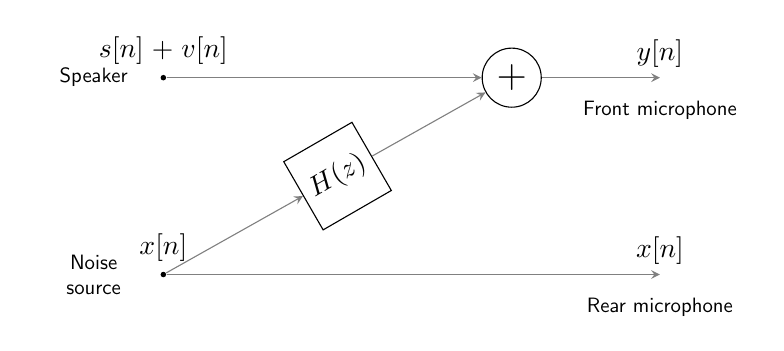
\begin{tikzpicture}[->, >=stealth, shorten >= 0pt, draw=black!50, node distance=2.5cm, font=\sffamily]
    \tikzstyle{node}=[circle,fill=black,minimum size=2pt,inner sep=0pt]
    \tikzstyle{block}=[draw=black,rectangle,fill=none,minimum size=1cm, inner sep=0pt]
    \tikzstyle{adder}=[draw=black,circle,fill=none,minimum size=0.75cm, inner sep=0pt]

	\node[node] (sc) {};
	\node[node, below of=sc] (xc) {};
	\node[adder, right=4cm of sc] (add) {\Large $+$};
	\coordinate (mid1) at ($(sc)!0.5!(add)$);
	\coordinate (mid2) at ($(sc)!0.5!(xc)$);
	
	\node[block, rotate=+30] (C) at (mid2 -| mid1) {$H(z)$};
	\coordinate[right=1.5cm of add] (yc) {};
	\coordinate[below of=yc] (yc2) {};
		
    \path (sc) edge (add);
    \path (xc) edge (yc2);
    \draw (xc) to (C.west);
    \draw (C.east) to (add);
    \draw (add) to (yc);
    
    \node[above = 0mm of sc, text width = 2.5cm, align=center] {$s[n]+v[n]$};
    \node[above = 0mm of yc, text width = 1cm, align=center] {$y[n]$};
    \node[above = 0mm of yc2, text width = 1cm, align=center] {$x[n]$};
    \node[below = 2mm of yc, text width = 3cm, align=center, scale=0.75] {Front microphone};
    \node[below = 2mm of yc2, text width = 3cm, align=center, scale=0.75] {Rear microphone};
    \node[left=0mm of xc, text width = 2cm, align=center, scale=0.75] {Noise  \\ source};
    \node[left=0mm of sc, text width = 2cm, align=center, scale=0.75] {Speaker};
    \node[above = 0mm of xc, text width = 1cm, align=center] {$x[n]$};
\end{tikzpicture}}
	\caption{Block diagram of noise canceling systems. For convenience, diagram uses discrete-time notation.}
	\label{fig:noise_cancelling_diagram1}
\end{figure}
\FloatBarrier

Figure~\ref{fig:noise_cancelling_diagram1} illustrates a diagram of this process. The speaker produces a signal $s[n] + v[n]$. $s[n]$ is the desired signal like a song, for instance. The signal $v[n]$ is the \textit{anti-noise} which will ideally cancel the noise perceived by the user and by the front microphone. The transfer function $H(z)$ is \underline{unknown} and it relates the noise in the rear microphone to the noise in the front microphone. To keep things simple, we will assume that $H(z)$ is \underline{time invariant}. Clearly, if we knew $H(z)$, we could make 
\begin{equation} \label{eq:v}
	v[n] = -h[n]\ast x[n] \implies y[n] \approx s[n]
\end{equation}

Therefore, the noise canceling problem boils down to estimating the filter $h[n] \Longleftrightarrow H(z)$.

To solve the following questions, you will need the files:

\begin{enumerate}
	\item \texttt{saw\_noise\_front\_mic.wav}: recording from the front microphone when $x[n]$ is the noise produced by a circular saw tool.
	\item \texttt{saw\_noise\_rear\_mic.wav}: recording from the rear microphone when $x[n]$ is the noise produced by a circular saw tool.
	\item \texttt{noise\_canceling.m}: this script loads the audio files and splits them into training and testing vectors. You should use the \texttt{*\_train} vectors for estimating the parameters and the \texttt{*\_test} vectors for testing your implementation.
\end{enumerate}

\begin{description}
	\item [(a)] (5 points) Show that when the signal $v[n]$ is not present, the cross-correlation between $y[n]$ and $x[n]$, $\phi_{yx}[m]$ is given by
	\begin{equation}
		\phi_{yx}[m] = \phi_{xx}[m]\ast h[m],
	\end{equation}
	where $h[m]$. Assume that the noise $x[n]$ and the signal $s[n]$ are uncorrelated. 
	
	\if\SOLUTIONS1 {\color{\SolutionsColor}
		
		\begin{align*}
		\phi_{yx}[m] &= \E(y[m]\ast x^*[-m]) \tag{definition} \\
		&= \E((s[m] + h[m]\ast x[m])\ast x^*[-n]) \tag{since $y[n] = s[n] + h[n]*x[n]$} \\
		&= \E(h[m]\ast x[m]\ast x^*[-m]) \tag{$s[n]$ and $x[n]$ are uncorrelated} \\
		&= h[m]\ast \E(x[m]\ast x^*[-m]) \tag{$h[n]$ is deterministic} \\
		&= h[m]\ast \phi_{xx}[m]
		\end{align*}
	}\fi
	
	\item [(b)] (3 points) Using the result from part (a), write an expression for $H(e^{j\omega})$ in terms of the PSD of $x[n]$ and in terms of $\Phi_{yx}[m] = \mathcal{F}\{\phi_{yx}[m]\}$.
	
	\if\SOLUTIONS1 {\color{\SolutionsColor} Convolution in time domain means multiplication in the frequency domain:
		\begin{align*}
		H(e^{j\omega}) = \frac{\Phi_{yx}(e^{j\omega})}{\Phi_{xx}(e^{j\omega})}
		\end{align*}
	}\fi
		
	\item[(c)] (7 points) Using any of the PSD estimation techniques covered in class, estimate the PSD of $x[n]$. Plot your estimate.
	
	\textit{Note:} to estimate the PSD, use the vectors \texttt{x\_train} and \texttt{y\_train} loaded by the script \texttt{noise\_canceling.m}.
	
	\if\SOLUTIONS1 {\color{\SolutionsColor} These solutions used the Blackman-Tukey method with Bartlett window of legnth 1023. This calculation could be performed using the function \texttt{blackman\_tukey\_psd.m} available on Canvas. See code for details. The plot is shown below.
		
		\FloatBarrier
		\begin{figure}[h!]
			\centering
			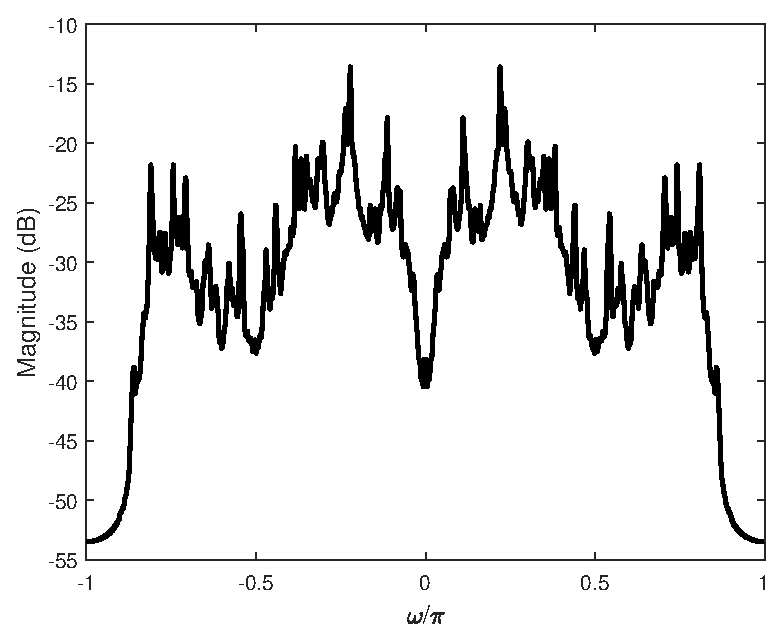
\includegraphics[scale=0.7]{figs/noise_cancel_x_psd.eps}
			\caption{$\Phi_{xx}(e^{j\omega})$ estimated using the Blackman-Tukey method.}
			\label{fig:noise_cancel_x_psd}
		\end{figure}
		\FloatBarrier
	}\fi
	
	\item[(d)] (7 points) Use the modified Blackman-Tukey PSD estimation method discussed in class to estimate $\Phi_{yx}(e^{j\omega}) = \mathcal{F}\{\phi_{yx}[m]\}$. Plot your estimate.

	\textit{Hint:} make sure to use \texttt{ifftshift} before computing the FFT in order to account for the indexing of the FFT.
	
	\if\SOLUTIONS1 {\color{\SolutionsColor} We can compute the Fourier transform of the cross-correlation function using the Blackman-Tukey algorithm as discussed in class:
		
		\begin{align*}
		&\texttt{phi\_yx\_hat = xcorr(y, x, M-1, 'unbiased')} \\
		&\texttt{s = phi\_yx\_hat.*window} \\
		&\texttt{S = fftshift(fft(ifftshift(s)))}
		\end{align*}
		
		Note that since the cross-correlation function is not necessarily even symmetric, using \texttt{abs()} or \texttt{real()} functions after the FFT calculation would produce incorrect results.
		
		The magnitude of the estimated $\Phi_{yx}(e^{j\omega})$ is shown in the plot below. See code for details.
			
		\FloatBarrier
		\begin{figure}[h!]
				\centering
				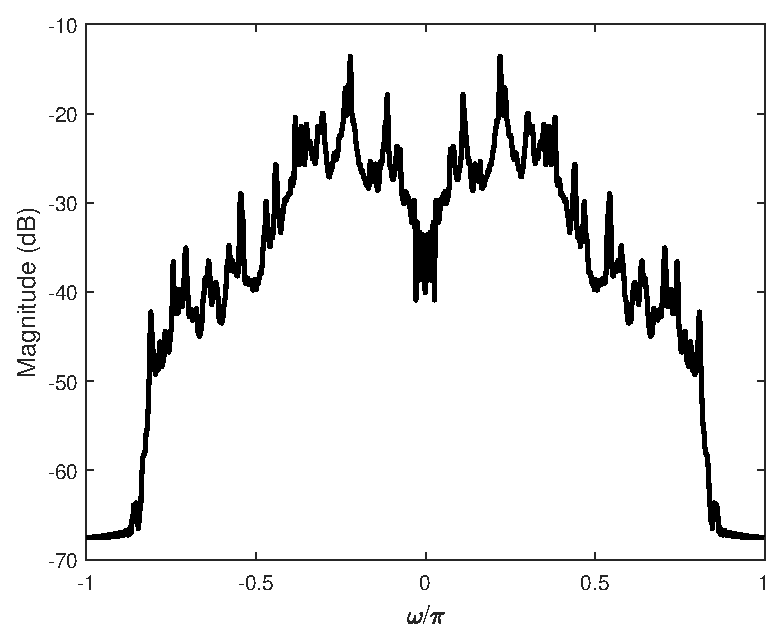
\includegraphics[scale=0.7]{figs/noise_cancel_cross_psd.eps}
				\caption{$\Phi_{yx}(e^{j\omega})$ estimated using the Blackman-Tukey method}
				\label{fig:noise_cancel_cross_psd}
		\end{figure}
		\FloatBarrier
		}\fi
	
	\item[(e)] (5 points) Combine your results from parts (b) through (d) to obtain an estimate for $H(e^{j\omega})$. Plot the magnitude response of $H(e^{j\omega})$ in dB.
	
	
	\if\SOLUTIONS1 {\color{\SolutionsColor} Combining the previous results yields
				
		\FloatBarrier
		\begin{figure}[h!]
			\centering
			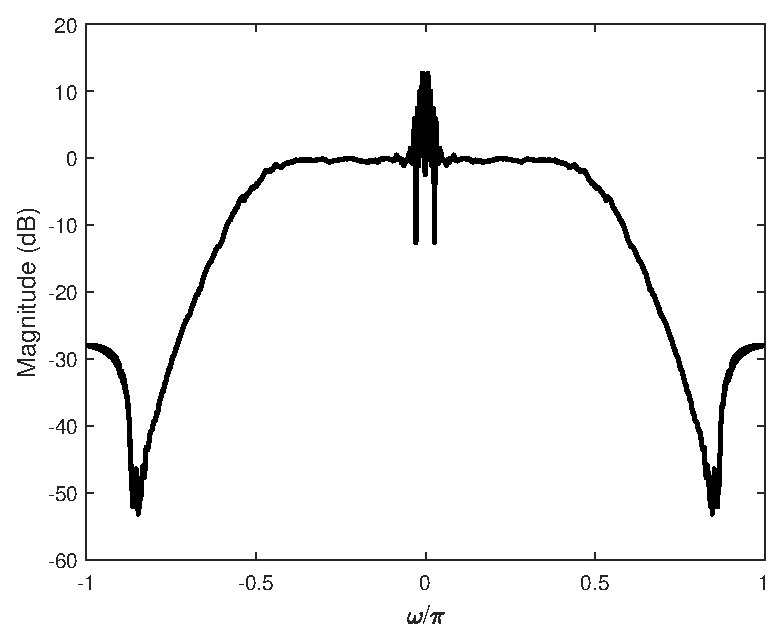
\includegraphics[scale=0.7]{figs/noise_cancel_Hest.eps}
			\caption{Magnitude of estimated $H(e^{j\omega})$.}
			\label{fig:noise_cancel_Hest}
		\end{figure}
		\FloatBarrier
	}\fi
	
	\item[(f)] (13 points) Use the leasts-squares method to design an FIR filter to approximate $H(e^{j\omega})$. Note that your filter \underline{does not} have to be linear phase, but it has to have \underline{real coefficients}. Additionally, your filter should have 50 coefficients. On the same graph, plot the magnitude of your filter and the magnitude of the desired response $H(e^{j\omega})$.
	
	\if\SOLUTIONS1 {\color{\SolutionsColor} Since the filter must have 50 coefficients, the order of the filter is $M = 49$. See code for design details. The figure below shows the magnitude of the FIR filter:
		\FloatBarrier
		\begin{figure}[h!]
			\centering
			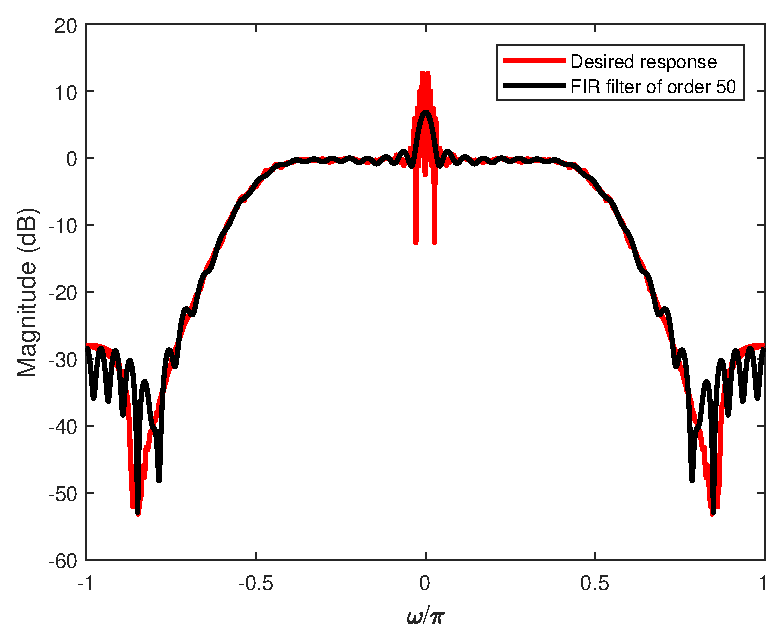
\includegraphics[scale=0.7]{figs/noise_cancel_Hfir.eps}
			\caption{Magnitude designed FIR filter.}
			\label{fig:noise_cancel_Hfir}
		\end{figure}
		\FloatBarrier	
	}\fi
	
	\item[(g)] (5 points) Use your filter to compute the signal $v[n]$ according to \eqref{eq:v} and use this result to remove the noise from the  signal $y[n]$. Specifically, define
	\begin{equation}
		y_{clean}[n] = y[n] + v[n].
	\end{equation}
	
	For these calculations, use the vectors \texttt{x\_test} and \texttt{y\_test} in the script \texttt{noise\_cancelling.m} to obtain the vector \texttt{y\_clean}. Use the function \texttt{sound} to play the new signal $y_{clean}[n]$ and comment on whether the noise was effectively canceled. 
	
	\if\SOLUTIONS1 {\color{\SolutionsColor} As indicated in the problem statement, we can make
		\begin{align*}
			&y_{clean}[n] = y[n] + v[n] = y[n] - h_{FIR}[n]\ast x[n] \\
			&\texttt{y\_clean = y\_val - filter(h\_FIR), 1, x\_val)}
		\end{align*}
		
		Although this does not result in perfect noise cancellation, it does improve the quality considerably.
	}\fi

\end{description}

\textbf{Note:} Although this noise canceling technique works well, in practice digital noise canceling systems use adaptive filters, since the cross-correlation computations used in this method require too much data to be accurate. However, this technique can always be applied to remove noise from one signal when we have two correlated measurements of the noise.

\if\SOLUTIONS1 
\subsection*{Code for Problem 2}
% This file was automatically created from the m-file 
% "m2tex.m" written by USL. 
% The fontencoding in this file is UTF-8. 
%  
% You will need to include the following two packages in 
% your LaTeX-Main-File. 
%  
% \usepackage{color} 
% \usepackage{fancyvrb} 
%  
% It is advised to use the following option for Inputenc 
% \usepackage[utf8]{inputenc} 
%  
  
% definition of matlab colors: 
\definecolor{mblue}{rgb}{0,0,1} 
\definecolor{mgreen}{rgb}{0.13333,0.5451,0.13333} 
\definecolor{mred}{rgb}{0.62745,0.12549,0.94118} 
\definecolor{mgrey}{rgb}{0.5,0.5,0.5} 
\definecolor{mdarkgrey}{rgb}{0.25,0.25,0.25} 
  
\DefineShortVerb[fontfamily=courier,fontseries=m]{\$} 
\DefineShortVerb[fontfamily=courier,fontseries=b]{\#} 
  
\noindent                                                                                  
 \hspace*{-1.6em}{\scriptsize 1}$  $\color{mgrey}#%% Noise canceling#\color{black}$$\\
 \hspace*{-1.6em}{\scriptsize 2}$  clear, $\color{mdarkgrey}$clc, close all$\color{black}$$\\
 \hspace*{-1.6em}{\scriptsize 3}$   $\\
 \hspace*{-1.6em}{\scriptsize 4}$  [y, Fs] = audioread($\color{mdarkgrey}$'saw_noise_front_mic.wav'$\color{black}$); $\color{mgrey}$% Fs is sampling frequency$\color{black}$$\\
 \hspace*{-1.6em}{\scriptsize 5}$  [x, Fs] = audioread($\color{mdarkgrey}$'saw_noise_rear_mic.wav'$\color{black}$);   $\\
 \hspace*{-1.6em}{\scriptsize 6}$  $\\
 \hspace*{-1.6em}{\scriptsize 7}$  N = floor(length(y)/2);$\\
 \hspace*{-1.6em}{\scriptsize 8}$  $\\
 \hspace*{-1.6em}{\scriptsize 9}$  y_train = y(1:N);$\\
 \hspace*{-2em}{\scriptsize 10}$  y_val = y(N+1:end);$\\
 \hspace*{-2em}{\scriptsize 11}$  x_train = x(1:N);$\\
 \hspace*{-2em}{\scriptsize 12}$  x_val = x(N+1:end);$\\
 \hspace*{-2em}{\scriptsize 13}$  $\\
 \hspace*{-2em}{\scriptsize 14}$  $\color{mgrey}#%% c) Estimate x[n] PSD#\color{black}$$\\
 \hspace*{-2em}{\scriptsize 15}$  M = 512;$\\
 \hspace*{-2em}{\scriptsize 16}$  L = 2*M-1;$\\
 \hspace*{-2em}{\scriptsize 17}$  window = bartlett(L);$\\
 \hspace*{-2em}{\scriptsize 18}$  dw = 2*pi/L;        $\color{mgrey}$% Nfft = L;$\color{black}$$\\
 \hspace*{-2em}{\scriptsize 19}$  w = -pi:dw:pi-dw;$\\
 \hspace*{-2em}{\scriptsize 20}$  $\\
 \hspace*{-2em}{\scriptsize 21}$  Pxx = blackman_tukey_psd(x_train, window, M);$\\
 \hspace*{-2em}{\scriptsize 22}$  $\\
 \hspace*{-2em}{\scriptsize 23}$  $\color{mgrey}$% Plot results$\color{black}$$\\
 \hspace*{-2em}{\scriptsize 24}$  figure, $\color{mdarkgrey}$box on, hold on$\color{black}$$\\
 \hspace*{-2em}{\scriptsize 25}$  plot(w/pi, 10*log10(Pxx), $\color{mdarkgrey}$'k'$\color{black}$, $\color{mdarkgrey}$'LineWidth'$\color{black}$, 2)$\\
 \hspace*{-2em}{\scriptsize 26}$  xlabel($\color{mdarkgrey}$'\omega/\pi'$\color{black}$, $\color{mdarkgrey}$'FontSize'$\color{black}$, 12)$\\
 \hspace*{-2em}{\scriptsize 27}$  ylabel($\color{mdarkgrey}$'Magnitude (dB)'$\color{black}$, $\color{mdarkgrey}$'FontSize'$\color{black}$, 12)$\\
 \hspace*{-2em}{\scriptsize 28}$  saveas(gca, $\color{mdarkgrey}$'../figs/noise_cancel_x_psd'$\color{black}$, $\color{mdarkgrey}$'epsc'$\color{black}$)$\\
 \hspace*{-2em}{\scriptsize 29}$  $\\
 \hspace*{-2em}{\scriptsize 30}$  $\color{mgrey}#%% d) Estimate cross-correlation #\color{black}$$\\
 \hspace*{-2em}{\scriptsize 31}$  $\color{mgrey}$% unbiased autocorrelation estimator$\color{black}$$\\
 \hspace*{-2em}{\scriptsize 32}$  phi_yx_hat = xcorr(y_train, x_train, M-1, $\color{mdarkgrey}$'unbiased'$\color{black}$);  $\\
 \hspace*{-2em}{\scriptsize 33}$  s = phi_yx_hat.*window; $\color{mgrey}$% windowing$\color{black}$$\\
 \hspace*{-2em}{\scriptsize 34}$  Phi_yx_hat = fftshift(fft(ifftshift(s))); $\\
 \hspace*{-2em}{\scriptsize 35}$  $\color{mgrey}$% Note: ifftshift ensures that Phi_yx_hat is not phase shifted due to FFT $\color{black}$$\\
 \hspace*{-2em}{\scriptsize 36}$  $\color{mgrey}$% indexing. Using abs() or real() would result in incorrect estimates$\color{black}$$\\
 \hspace*{-2em}{\scriptsize 37}$  $\\
 \hspace*{-2em}{\scriptsize 38}$  $\color{mgrey}$% Plot results$\color{black}$$\\
 \hspace*{-2em}{\scriptsize 39}$  figure, $\color{mdarkgrey}$box on, hold on$\color{black}$$\\
 \hspace*{-2em}{\scriptsize 40}$  plot(w/pi, 10*log10(abs(Phi_yx_hat)), $\color{mdarkgrey}$'k'$\color{black}$, $\color{mdarkgrey}$'LineWidth'$\color{black}$, 2)$\\
 \hspace*{-2em}{\scriptsize 41}$  xlabel($\color{mdarkgrey}$'\omega/\pi'$\color{black}$, $\color{mdarkgrey}$'FontSize'$\color{black}$, 12)$\\
 \hspace*{-2em}{\scriptsize 42}$  ylabel($\color{mdarkgrey}$'Magnitude (dB)'$\color{black}$, $\color{mdarkgrey}$'FontSize'$\color{black}$, 12)$\\
 \hspace*{-2em}{\scriptsize 43}$  saveas(gca, $\color{mdarkgrey}$'../figs/noise_cancel_cross_psd'$\color{black}$, $\color{mdarkgrey}$'epsc'$\color{black}$)$\\
 \hspace*{-2em}{\scriptsize 44}$  $\\
 \hspace*{-2em}{\scriptsize 45}$  $\color{mgrey}#%% e)#\color{black}$$\\
 \hspace*{-2em}{\scriptsize 46}$  Hest = Phi_yx_hat./Pxx;$\\
 \hspace*{-2em}{\scriptsize 47}$  $\\
 \hspace*{-2em}{\scriptsize 48}$  $\color{mgrey}$% Plot results$\color{black}$$\\
 \hspace*{-2em}{\scriptsize 49}$  figure, $\color{mdarkgrey}$box on, hold on$\color{black}$$\\
 \hspace*{-2em}{\scriptsize 50}$  plot(w/pi, 20*log10(abs(Hest)), $\color{mdarkgrey}$'k'$\color{black}$, $\color{mdarkgrey}$'LineWidth'$\color{black}$, 2)$\\
 \hspace*{-2em}{\scriptsize 51}$  xlabel($\color{mdarkgrey}$'\omega/\pi'$\color{black}$, $\color{mdarkgrey}$'FontSize'$\color{black}$, 12)$\\
 \hspace*{-2em}{\scriptsize 52}$  ylabel($\color{mdarkgrey}$'Magnitude (dB)'$\color{black}$, $\color{mdarkgrey}$'FontSize'$\color{black}$, 12)$\\
 \hspace*{-2em}{\scriptsize 53}$  saveas(gca, $\color{mdarkgrey}$'../figs/noise_cancel_Hest'$\color{black}$, $\color{mdarkgrey}$'epsc'$\color{black}$)$\\
 \hspace*{-2em}{\scriptsize 54}$  $\\
 \hspace*{-2em}{\scriptsize 55}$  $\color{mgrey}#%% f) Filter design#\color{black}$$\\
 \hspace*{-2em}{\scriptsize 56}$  M = 49;$\\
 \hspace*{-2em}{\scriptsize 57}$  $\\
 \hspace*{-2em}{\scriptsize 58}$  $\color{mgrey}$% Calculate matrix Q$\color{black}$$\\
 \hspace*{-2em}{\scriptsize 59}$  $\color{mgrey}$% This assumes even symmetry$\color{black}$$\\
 \hspace*{-2em}{\scriptsize 60}$  Q = zeros(length(w), M+1); $\color{mgrey}$% initialized$\color{black}$$\\
 \hspace*{-2em}{\scriptsize 61}$  n = 0:M; $\color{mgrey}$% time vector$\color{black}$$\\
 \hspace*{-2em}{\scriptsize 62}$  $#for#$ i = 1:length(w) $\color{mgrey}$% for every frequency wi$\color{black}$$\\
 \hspace*{-2em}{\scriptsize 63}$      Q(i, $\color{mdarkgrey}$:) = exp(-1j*w(i)*n);$\color{black}$$\\
 \hspace*{-2em}{\scriptsize 64}$  $#end#$$\\
 \hspace*{-2em}{\scriptsize 65}$  $\\
 \hspace*{-2em}{\scriptsize 66}$  $\color{mgrey}$% Least-squares algorithm$\color{black}$$\\
 \hspace*{-2em}{\scriptsize 67}$  d = Hest;$\\
 \hspace*{-2em}{\scriptsize 68}$  hls = real(pinv(Q)*d); $\color{mgrey}$% real() removes imaginary part due to numerical errors$\color{black}$$\\
 \hspace*{-2em}{\scriptsize 69}$  Hls = freqz(hls, 1, w);$\\
 \hspace*{-2em}{\scriptsize 70}$  $\\
 \hspace*{-2em}{\scriptsize 71}$  $\color{mgrey}$% Plot results$\color{black}$$\\
 \hspace*{-2em}{\scriptsize 72}$  figure, $\color{mdarkgrey}$box on, hold on$\color{black}$$\\
 \hspace*{-2em}{\scriptsize 73}$  plot(w/pi, 20*log10(abs(Hest)), $\color{mdarkgrey}$'r'$\color{black}$, $\color{mdarkgrey}$'LineWidth'$\color{black}$, 2)$\\
 \hspace*{-2em}{\scriptsize 74}$  plot(w/pi, 20*log10(abs(Hls)), $\color{mdarkgrey}$'k'$\color{black}$, $\color{mdarkgrey}$'LineWidth'$\color{black}$, 2)$\\
 \hspace*{-2em}{\scriptsize 75}$  legend($\color{mdarkgrey}$'Desired response'$\color{black}$, $\color{mdarkgrey}$'FIR filter of order 50'$\color{black}$)$\\
 \hspace*{-2em}{\scriptsize 76}$  xlabel($\color{mdarkgrey}$'\omega/\pi'$\color{black}$, $\color{mdarkgrey}$'FontSize'$\color{black}$, 12)$\\
 \hspace*{-2em}{\scriptsize 77}$  ylabel($\color{mdarkgrey}$'Magnitude (dB)'$\color{black}$, $\color{mdarkgrey}$'FontSize'$\color{black}$, 12)$\\
 \hspace*{-2em}{\scriptsize 78}$  saveas(gca, $\color{mdarkgrey}$'../figs/noise_cancel_Hfir'$\color{black}$, $\color{mdarkgrey}$'epsc'$\color{black}$)$\\
 \hspace*{-2em}{\scriptsize 79}$  $\\
 \hspace*{-2em}{\scriptsize 80}$  $\color{mgrey}#%% g)#\color{black}$$\\
 \hspace*{-2em}{\scriptsize 81}$  y_clean = y_val - filter(hls, 1, x_val);$\\
 \hspace*{-2em}{\scriptsize 82}$  sound(y_clean, $\color{mdarkgrey}$Fs)$\color{black}$$\\ 
  
\UndefineShortVerb{\$} 
\UndefineShortVerb{\#}
\fi


\end{document}
